\documentclass[fleqn,10pt]{wlscirep}
\usepackage[utf8]{inputenc}
\usepackage[T1]{fontenc}
\title{Reduced Exploratory behavior in cue-poor but not cue-rich open-field environments in TgF344-Alzheimer’s disease rats}

\author[1,*]{Laura E. Berkowitz}
\author[1]{Elizabeth A. Sneddon}
\author[1]{Ryan E. Harvey}
\author[1]{Maria Gabaldon-Parish}
\author[1]{M\^{o}nica Gon\c{c}alves-Garcia}
\author[1,*]{Benjamin J. Clark}
\affil[1]{University of New Mexico, Psychology, Albuquerque, NM 87131, United States}

\affil[*]{bnjclark@unm.edu, lberkowitz@unm.edu}

\keywords{Exploratory behavior, Home base, Alzheimer’s disease, Open-field, Spatial Navigation}

\begin{abstract}
Spatial navigation is impaired in the early stages of Alzheimer’s disease (AD). This impairment is thought to arise from a deficit in transitioning between or using cues within two key reference frames; allocentric (body independent) and egocentric (body dependent). Use of cues for navigation within the allocentric reference frame becomes impaired in AD very early in disease progression. Studies of exploratory behaviors in rodents may reveal how these cue-cue or cue-body relationships form by tracking the behaviors of rodents in an open field environment denoted with a proximal cue. The TgF344-AD rat model of AD has been shown to develop a comprehensive profile of AD pathology which progressively worsens performance in spatial memory tasks. However, it is currently unknown how TgF344-AD rats gather spatial information during open-field exploration. We examined exploratory behaviors in TgF344-AD rats and F344 controls in cue-poor and and cue-rich environment. TgF344-AD rats showed reduced exploration in the cue-poor environment starting at 11-12 months of age, but showed no differences in exploration in a cue-rich environment at 13 months. TgF344-AD rats also showed similar interaction with a local cue compared to F344 controls. These results highlight the importance of environmental context on exploratory behaviors in rodent models of Alzheimer's disease.   


% Exploratory behaviors were assessed in the presence of a proximal cue and 24 h later once the cue was removed. Results indicate that TgF344-AD rats and controls shared similar locomotion and exploratory behaviors. Additionally, both groups established home bases, although the location of the home bases was equally variable between days across both groups. Overall, this study indicates that TgF344-AD rats at 13 months of age show similar spatial memory and exploratory behaviors found in F344 controls. 
\end{abstract}

\begin{document}

\flushbottom
\maketitle
% * <john.hammersley@gmail.com> 2015-02-09T12:07:31.197Z:
%
%  Click the title above to edit the author information and abstract
%
\thispagestyle{empty}

\section*{Introduction}

Alzheimer’s disease (AD) is characterized by a progressive accumulation of amyloid plaques and neurofibrillary tangles resulting in neurodegeneration of key medial temporal lobe structures involved in spatial navigation. One of the earliest deficits observed in AD involves an inability to accurately navigate. Experimentally, these deficits are apparent in tasks that require locating hidden goals, where individuals with prodromal Alzheimer's disease have longer paths when navigating to a hidden goal location. Animal models of AD-like pathology have shown similar navigation deficits in rodent analogues of this task \cite{berkowitz_progressive_2018,janus_search_2004}. Successful navigation in these tasks usually points to the use of environmental cues, usually prominent polarizing landmarks, as rotation or removal of these cues shows corresponding changes in navigation patterns \cite{}. 

An understanding of how animals use environmental cues for navigation has been approached by tracking the behaviors of rodents in open environments \cite{dudchenko_neuroethology_2018,poulter_neurobiology_2018,thompson_behavioral_2018}. For instance, when placed in an open field, rats organize their exploratory behaviors around particular locations, called home bases. At these locations, rats spend a disproportionate amount of time, perform prolonged crouching, grooming, circling, and rearing movements \cite{eilam_home_1989}, and make slow exploratory excursions into the remaining environment, followed by direct, rapid returns to the home base \cite{wallace_nmda_2003}. Although rats express home base behavior in relatively featureless environments and in darkness \cite{eilam_home_1989,hines_home_2005,nemati_point_2007}, they establish their bases near landmarks that offer security such as shelters, walls, or prominent visual cues \cite{clark_impaired_2005,hines_home_2005,lehmann_complete_2007,wallace_nmda_2003,whishaw_exploratory_2006}. If the landmark is displaced, animals tend to return and dwell near the previously cued base location, suggesting the retention of spatial information acquired during exploration \cite{clark_impaired_2005,hines_home_2005,lehmann_complete_2007}(Clark et al., 2006; Hines \& Whishaw, 2005; Lehmann et al., 2007; Travis et al., 2010). 

While the TgF344-AD rat model shows promise for the study of spatial navigation impairments \cite{berkowitz_progressive_2018}, very little is known regarding changes in open field behavior.  The present study includes a longitudinal assessment of open field behavior following male and female rats at four time-points. Rats were allowed to explore a small open field environment at 4-5, 7-8, and 10-12 months of age over the course of three days. At 12-13 months of age, rats were placed individually onto a large open circular table top and were allowed to explore for 30 minutes for two consecutive days. In this environment, a proximal cue was positioned on the edge of the table on Day 1, which served to bias the formation of a home base at that location. On Day 2, the proximal cue was removed from the open field. Results indicate that TgF344-AD rats show progressive reduction in locomotion in a small open field environment with significant reductions at 12 months of age compared to F344 wild type controls, including having shorter path lengths and exploring a smaller proportion of the open field environment. Additionally, both TgF344-AD and F344 rats showed variable preference in using the proximal cue for establishing a home base and responded similarly to the removal of the proximal cue during the probe test. Overall, these results indicate relatively intact exploratory behavior in TgF344-AD rats at 13 months.   

\section*{Results}

\subsection*{Longitudinal small open field assessment}

TgF344-AD rats develop progressive pathology within the hippocampus, which has been reported as early as 6 months of age \cite{cohen_transgenic_2013}. These pathological changes may contribute to disruptions in hippocampal function of TgF344-AD rats \cite{stoiljkovic_altered_2018}. We thus sought to determine whether TgF344-AD rats exhibit changes in exploratory and habituation behaviors that are associated with hippocampal disruption. Animals were examined for 10 minutes within a small open field environment across three time points (4-5 months, 7-8 months, 10 - 12 months), and over three consecutive days. 

\subsubsection*{TgF344-AD rats have reduced locomotion starting at 12 months of age}
We first sought to determine whether animals exhibited behaviors consistent with habituation, such as reduced locomotion across days or across days and time points. Measures of locomotion consisted of total distance traveled (or path length (cm)), running speed (cm/s), and percent of the arena explored. We found that TgF344-AD and WT controls exhibited similar locomotion across days, though TgF344-AD animals moved less as they aged compared to control animals. Specifically, TgF344-AD animals exhibited decreased path length and decreased median velocity compared to WT controls at 10 - 12 months of age ($\beta$ = 1.072, p =  0.0348 and $\beta$ = 0.010, p = 0.0040, respectively (Fig\ref{locomotor_fig}b,c)).  Furthermore, TgF344-AD animals tended to explore a lower proportion of the environment compared to control animals,($\beta$ = 0.047, p = 2.23e-06), though this was not significantly different across time,($\beta$ = 0.012, p = 0.074)(Fig\ref{locomotor_fig}b). All animals spent progressively more time at the perimeter of the open field, spending an average of 83$\%$ of the session at the perimeter at 7 months ($\beta$ = 5.80e08, p = 5.07e-13)  and 89$\%$ of the session at the perimeter at 12 months ($\beta$ = 4.01e08, p = < 2e-16)(Fig\ref{locomotor_fig}d). Thus, TgF344-AD rats exhibited a progressive decrease in locomotion at 12 months of age and overall tended to explore a smaller proportion of the open field environment compared to control animals. 

\subsubsection*{TgF344-AD rats stop less frequently and have longer stop duration}   
Disruption of hippocampal function is associated with altered stopping behaviors during exploration \cite{martin_medial_2007}. We thus tested the hypothesis that TgF344-AD animals would make more frequent and shorter stops. Overall, TgF344-AD rats tended to make a fewer number of stops than control animals, ($\beta$ = 0.258, p = 7.79e-05), while both groups tended to make fewer stops on day 1 compared to day 2, ($\beta$ = 0.190, p = 0.0151). As animals aged, their stops tended to increase in duration, with animals having longer stops at 7 months of age compared to 4 months of age, ($\beta$ = 0.111, p = 0.000126), and at 12 months of age compared to the previous ages, ($\beta$ = 0.077, p = 4.64e-06). Overall, TgF344-AD rats tended to have longer stops and longer time between stopping compared to controls ($\beta_s \leq$ -0.034, ps $\leq$ 0.048).

\subsubsection*{Both TgF344-AD and control rats exhibit unstable home base locations across days}
We next investigated whether TgF344-AD and WT control rats established home bases in the open field. Home base behaviors are organized around a specific location where the rat spends a disproportionate amount of time \cite{tchernichovski_part_nodate}. Briefly, home bases were defined as high occupancy regions where the rat moved slowly for at least 70$\%$ of the time spent in that region. The home base with the maximum occupancy was defined as the primary home base. TgF344-AD and control animals established primary home bases along the wall of the open field, with controls having a slightly closer a mean distance to the wall(4.25 cm vs 4.84 cm, $\beta$ = 0.28, p = 0.011). In addition, the primary home base moved closer to the wall across time points, ($\beta_s \leq$ -0.299, ps $\leq$ 0.014). We also examined the latency to visit the primary home base location. While there were no group differences, latency to reach the primary home base was increased at 10 - 12 months of age compared to the two prior time points, ($\beta$ = 9.476, p = 0.015). Overall, TgF344-AD rats spent more time in their primary home base compared to control rats (188 sec vs 151 sec, respectively, $\beta$ = 0.145, p = 0.002), and all rats progressively spent more time in their primary home base across time points, ($\beta_s \leq$ -0.092, ps $\leq$ 0.040). 

We next asked whether TgF344-AD rats and controls primary home base maintained a similar position in the open field across days. To examine this, the mean distance between primary home base centroids was calculated across all three days. Overall, home base distances exhibited a left-skewed distribution that ranged from 5.1 cm to 59.4 cm. All rats tended to move their primary home base over days as indicated by a median distance of 44.4 cm. At 4 - 5 months of age, TgF344-AD rats tended to have primary home bases that were closer together compared to controls, (31.1 cm vs. 52.2 cm, respectively, $\beta$ = 37.912, p = 0.033). 

\begin{figure}
    \centering
    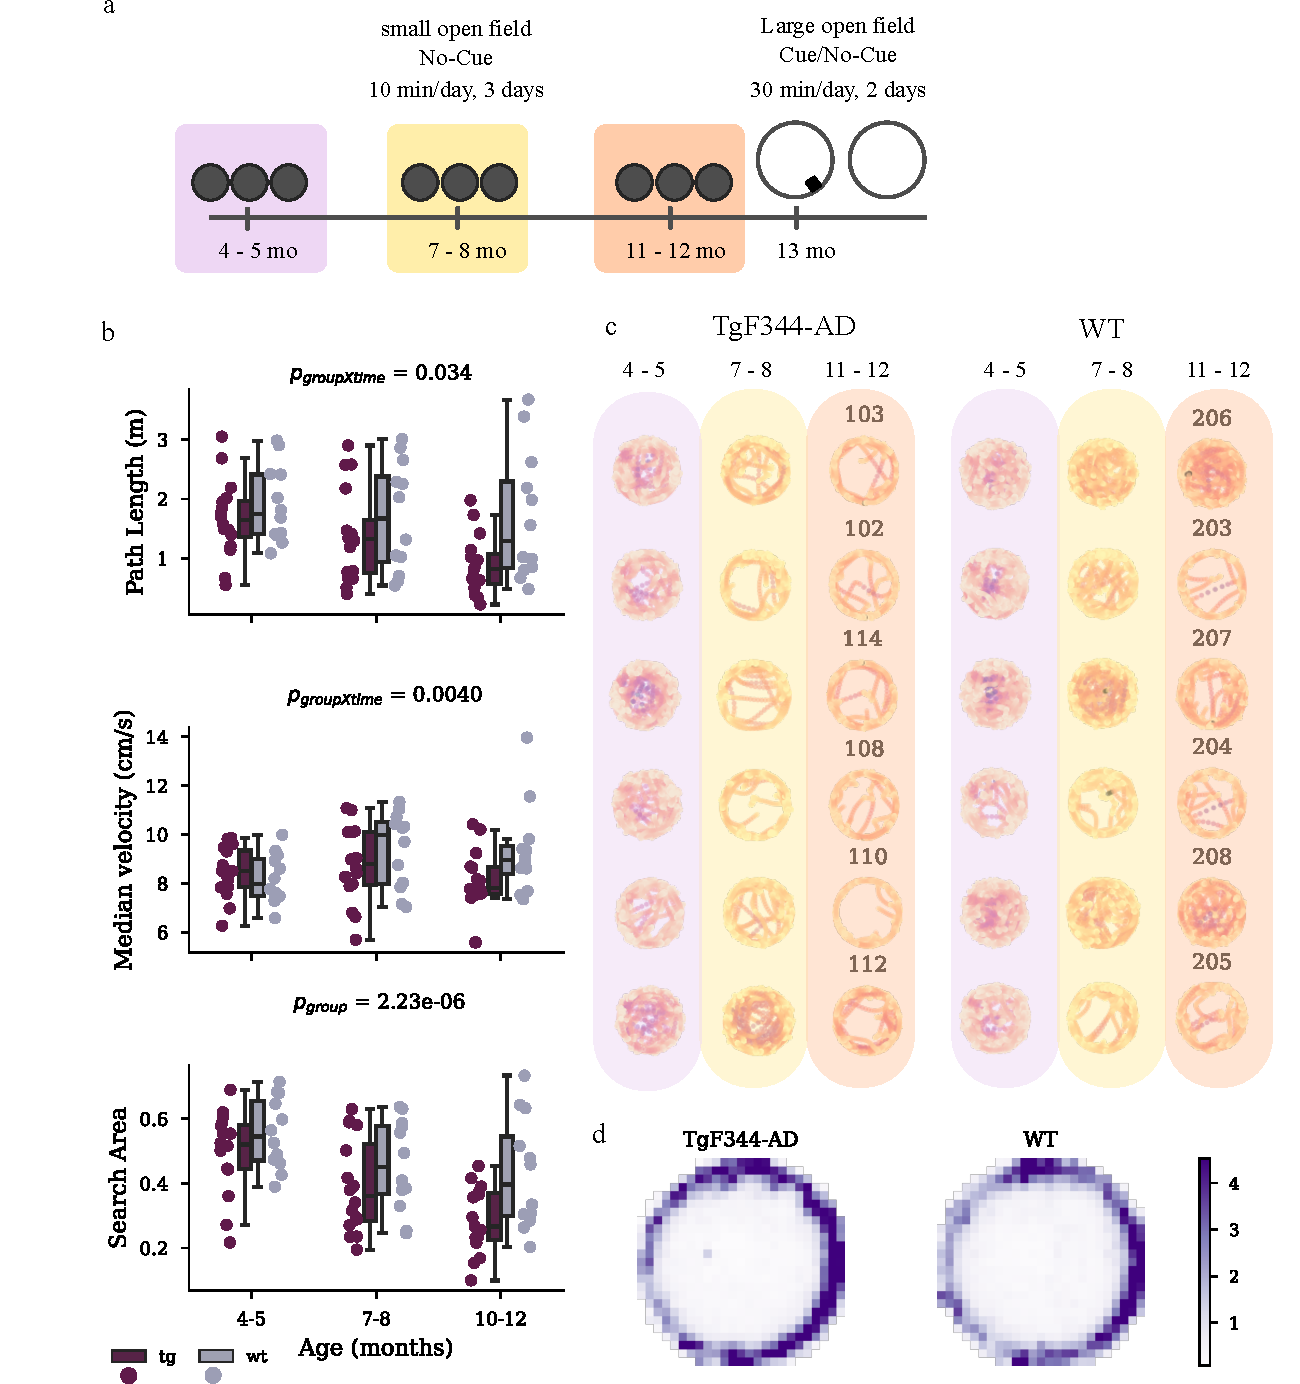
\includegraphics[width=1\textwidth]{notebooks/figs/Figure1.pdf}
    \caption{TgF344-AD rats exhibit reduced open field exploration at 11 - 12 months. a) Schematic of longitudinal organization of open field experiments. b) Stripplot and boxplots summarizing locomotion measures for the small open field tests over time. Points represent daily averages for each subject within a time point. P-values for significant effects observed in the interaction linear models including group and time-point as factors. c) Example paths for six animals from each group. Paths for all three days are plotted for a given time-point. Path points are color coded by the animals velocity with deeper purple tones representing fast path segments. d) Heat-maps reflecting the occupancy in the small open field across all days and time-points for each group. Note that all animals spend the majority of their time by the wall.}
    \label{locomotor_fig}
\end{figure}


\subsection*{Influence of proximal cue on home base preference}
Rats establish a home base in locations adjacent to a proximal or salient visual cue \cite{nemati_point_2007,hines_home_2005}. We tested whether TgF344-AD rats are able to establish a home base preference relative to a proximal cue after a single exposure, and examined this preference the next day following cue removal. Briefly, TgF344-AD and control rats were exposed to a novel open field environment for 30 minutes across two days. A proximal cue was positioned on the outer edge of the maze and was removed the following day to test whether home bases were established in the region adjacent to the proximal cue's previous location. No difference in locomotion or stopping behaviors was observed between groups, indicating that the animals exhibited similar exploratory behaviors in a large open field environment (see Supplemental table X).

\subsubsection*{Cue Interaction} 
We first measured the interaction with the proximal cue, as previous studies suggest that rats tend to explore and frequently stop around a proximal cue \cite{hines_home_2005,lehmann_complete_2007}. The majority of rats from both groups visited the proximal cue at least once (TgF344-AD: 75 $\%$ (9/12), controls: 75 $\%$ (9/12)), and those rats that visited the cue did so within 90 seconds on day 1, and within 30 seconds on day 2, ($\beta$ = -1.069, p = 0.022), suggesting that rats that explored the proximal cue were able to form an object-place association after one exposure. 

\begin{figure}
    \centering
    \includegraphics[width=1\textwidth]{}
    \caption{Caption}
    \label{homebase_fig}
\end{figure}

\subsubsection*{Home Base} 
We next investigated whether TgF344-AD and WT control rats established a primary home base near the proximal cue location. There is a clear bimodal distribution, whereby some rats set up their primary home base near the cue (< 25cm) while other rats set up home bases nearly a meter or more from the cue boundary. Although TgF344-AD rats tended to establish a home base further from the cue boundary relative to WT controls (TgF344-AD median: 121 cm vs WT median 11cm), there was no significant difference in median home base distance from cue between groups  ($X^2(1)$  = 1.094, p = 0.29). Overall, these results indicate that there was a mixed preference in using the proximal cue to establish a home base location for either group. 

\subsubsection*{Probe Test: Proximal Cue Removal}
Previous work has shown that rats respond to the novelty of cue removal with frequent visits to the previously cued location typically within the first several minutes of testing \cite{hines_home_2005}(Hines et al., 2005; Travis et al., 2010). Only 50\% of TgF344-AD and 66\% of Wt rats entered the previously cued location at least once ($X^2(1)$ = 0.17, p = 0.67). Furthermore, both groups stopped at the previously cued location and the number of stops at this location did not differ between groups ($X^2(1)$ = 1.27, p = 0.25). Although the median latency to reach the cued location was lower in TgF344-AD rats (4.31 s) compared to WT controls (20.7 s), this was not significantly different, ($X^2(1)$ = 3.12, p = 0.07). 
 
We next sought to identify whether rats returned to their primary home base location on day one. The distance between the center of the primary home base was computed across days. Median distances between primary home bases between days suggested that TgF344-AD rats tend to make home bases nearer the previous day’s location (TgF344-AD: 47.1 cm), although this was not significantly different than controls (WT: 116.2 cm) ($X^2(1)$ = 1.92, p = 0.16).  


% In general, most rats in both groups exhibited a clear preference for a location in the open field. In many cases, rats established more than one home base with the median number of home bases similar between groups ($X^2(1)$ = 0.93, p = 0.33). TgF344-AD rats and WT controls visited their primary home base location, defined as the home base with the greatest occupancy, within the first 2-3 minutes. Again, the elapsed time to primary home base establishment did not significantly differ between groups ($X^2(1)$ = 0.31, p = 0.57). Furthermore, no differences were observed between groups for the duration of time spent in the primary home base (t(22) = 0.73, p = 0.46) nor the number of stops made in the primary home base ($X^2(1)$  = 1.59, p = 0.20). Thus, home base behaviors were similar between TgF344-AD and WT controls. 

% Proximal or salient visual cues have been shown to influence where a home base is established \cite{nemati_point_2007,hines_home_2005}. Thus, we sought to identify whether rats established home bases near the proximal cue by calculating the distance between the primary home base center and the closest edge to the proximal cue. 


% \subsection*{Probe Test: Proximal Cue Removal}
% Twenty-four hours after the open field test, a probe test was conducted in which the rats were returned to the open field but with the proximal cue removed from the environment. Difference scores were computed to determine whether behavior change was different between groups across days. Changes in behaviors including locomotor distance, exploration area, linear speed, linear acceleration, angular velocity during exploration, angular velocity during stops, number of run epochs, or number of stops changed to the same extent between groups (supplemental Table X). 

% Previous work has shown that rats respond to the novelty of cue removal with frequent visits to the previously cued location typically within the first several minutes of testing \cite{hines_home_2005}(Hines et al., 2005; Travis et al., 2010). Only 50\% of TgF344-AD and 66\% of Wt rats entered the previously cued location at least once ($X^2(1)$ = 0.17, p = 0.67). Furthermore, both groups stopped at the previously cued location and the number of stops at this location did not differ between groups ($X^2(1)$ = 1.27, p = 0.25). Although the median latency to reach the cued location was lower in TgF344-AD rats (4.31 s) compared to WT controls (20.7 s), this was not significantly different, ($X^2(1)$ = 3.12, p = 0.07). 

% We next sought to identify whether rats returned to their primary home base location on day one. The distance between primary home bases between days was computed for each rat. Median distances between primary home bases between days suggested that TgF344-AD rats tend to make home bases nearer the previous day’s location (TgF344-AD: 47.1 cm), although this was not significantly different than controls (WT: 116.2 cm) ($X^2(1)$ = 1.92, p = 0.16). 

% Overall, these results indicate that the removal of a proximal cue influences the behaviors of TgF344-AD and Wt rats similarly during open field exploration. 

\section*{Discussion}

This experiment identified that exploratory and home base behaviors are similar between TgF344-AD rats and F344 (WT) controls at 13 months. On an open-field, TgF344-AD rats travel similar distances and explore similar proportions of the total maze as WT controls. In addition, we found no differences in average linear or angular velocities between these groups. Segmenting paths into excursions indicated that TgF344-AD rats tend to travel in more direct paths in between stops, whereas WT rats tend to have a greater extent of meandering. Nevertheless, the frequency of excursions and the median duration of these excursions is comparable between TgF344-AD and WT rats. Analysis of stopping behavior revealed that the median stop duration for TgF344-AD rats was shorter than that of WT rats, yet the frequency of total stops made were similar between groups. Additionally, TgF344-AD rats established home bases and spent a similar amount of time in their primary home base as WT rats. Interestingly, both TgF344-AD and WT rats showed split influence of a proximal visual cue in determining their primary home base location, whereby the proximity of the primary home base to the cue location resembled a bimodal distribution for both groups. Overall, TgF344-AD rats show few differences in locomotor behavior while responding to environmental features and when establishing a home base at 13 months compared to WT controls. 


These analyses expand upon prior assessments of open-field behaviors in TgF344-AD rats. Locomotion measures reported in previous open field experiments involving TgF344-AD rats have largely focused on gross metrics of movement such as distance travelled \cite{morrone_regional_2020,voorhees_occupational-like_2019,voorhees_-p7c3-s243_2018} or beam breaks \cite{cohen_transgenic_2013}, while limiting observations to 10 minutes of open field exploration. While these metrics hold value in understanding the extent of movement during exploration, they provide an incomplete profile of how TgF344-AD rats explore novel, open environments. This study expanded the locomotion profile of TgF344-AD rats by examining kinematic attributes, including linear velocity/acceleration, angular acceleration, and features of movement segments and stops. Kinematic analyses have shown to be powerful discriminators of strain or genotype \cite{benjamini_ten_2010}. Furthermore, evaluations of kinematic profiles of excursions or incursions from a home base have been implicated in supporting dead reckoning, or the ability to locate a point of departure by continuously updating the current position through the integration of self-motion cues \cite{wallace_fractionating_2008,wallace_movement_2006,wallace_quantification_2002}.


The kinematic profile of TgF344-AD rats largely resembled that of WT control rats except in regard to stop duration and circuity of movement segments. TgF344-AD rats tended to stop for a shorter duration compared to control animals. Similarly, short duration stops have been observed in Fimbria-Fornix lesioned animals \cite{whishaw_short-stops_1994}. However, it is currently unknown whether Fimbria-Fornix function is altered in TgF344-AD rats; thus, future work should explore the pathology in this region or examine the functional connectivity between regions connected by this fiber pathway. 
Home base behaviors were found to be similar between TgF344-AD rats and WT controls.

It is possible that the similar locomotor behavior may be due to anxiety-like behavior exhibited by both groups of subjects. One limitation is that these rats were tested during the dark cycle in a well-lit room. Rodents typically prefer dark, enclosed spaces (CITE) therefore it is likely that all subjects may have exhibited heightened anxiety-like behavior throughout the task. Although this is a concern that should be taken into consideration, all subjects were exposed to the same environmental conditions, therefore it is unlikely that an increase in anxiety-like behavior was the driving factor behind the observed behaviors. 

Emphasize Fisher 344 model and normal aging and exploratory behavior assessment

Overall, the results of this study indicate only subtle changes to locomotion and intact home base behavior in TgF344-AD rats. This indicates that exploratory behaviors may not contribute to observed spatial navigation deficits found in TgF344-AD rats \cite{berkowitz_progressive_2018}. 

\section*{Methods}

\subsection*{Subjects} 
Twelve TgF344-AD rats counterbalanced for sex and expressing mutant human amyloid precursor protein (APPsw) and presenilin 1 (PS1$\Delta$E9) were obtained directly from the Rat Resource \& Research Center (Columbia, MO). Twelve wild type Fischer 344 (WT) rats (Harlan laboratories, Indianapolis, IN) counterbalanced for sex served as control subjects. Subjects were maintained under controlled temperature (21 $\pm$ 2 $^{\circ}$C), were housed with TgF344-AD or WT pairs, and were kept on a 12-hour light/dark cycle (lights off at 09:00 AM). Food and water was provided \textit{ad libitum} throughout the duration of the study. Furthermore, all animals were part of a longitudinal study assessing various behavioral phenotypes, some of which have been reported previously \cite{berkowitz_progressive_2018,pentkowski_anxiety-like_2018}. Thus, all animals had extensive handling and prior experience in both wet and dry maze experiments starting at 4 months of age. Animal care practices and experiments were approved by the University of New Mexico Institutional Animal Care and Use Committee.

\subsection*{Testing Room}
Testing took place in a large, white, well-lit room. Located in the room was a table with a computer, a table with a white noise machine, a cabinet, a trash can, a paper towel dispenser, and a sink. A video camera was mounted above the open field apparatus. Video data was collected for all experiments. Prior to each behavioral test, the white noise machine was turned on to cancel out outside noise.

\subsection*{Apparatus and Proximal Cue}
The open field apparatus consisted of a large circular table made of wood (202 cm in diameter). The table was painted white and rested on a platform that was 24 cm from the floor. A Styrofoam box 27.5 cm X 22.5 cm X 18.5cm was painted black and served as the proximal cue. The proximal cue occupied a fixed location in the room with respect to the distal room cues. The table and Styrofoam box were cleaned with a Virex solution between testing sessions of each rat to control for odor cues between rats. 

\subsection*{Behavior Testing Procedures}

\subsubsection*{Open Field Test} To assess exploratory behavior, rats underwent a single exposure to the large open field. Eight hours into the dark cycle (5:00 PM), rats were weighed in the colony room prior to behavioral testing, were carried to the testing room in a plastic box, and placed in the center of the open field. Each individual testing session lasted 30 minutes. The experimenter stayed in the room during all experimental testing and only interacted with the subjects to replace them on the open field apparatus if they fell or jumped off the apparatus. After each testing session, rats were returned to their home cage then returned to the colony room by 9:00 PM (before lights on).

\subsubsection*{Probe Test: Proximal Cue Removal} Approximately 24 hours after the open field test, rats underwent the same procedure as described above except the the proximal cue was removed from the maze.  


\subsection*{Data Analysis}
\subsubsection*{Movement Tracking}The location of each rat on the open field was tracked offline using DeepLabCut2.85b (for detailed review of methods see \cite{mathis_deeplabcut_2018}. Briefly, 480 images were obtained from eight of the 48 recorded task videos. For each image, an experimenter marked the nose, head (in between ears), back (middle of torso), and base of tail. Using the trainnetwork function, the labelled images were then used to train the network over 200,000 iterations or until results from the evaluatenetwork function to verify the labelling accuracy was less than 3 cm. Once the accuracy threshold was met, the network was then used to label all recorded task videos. The output from DeepLabCut was then brought into Matlab for further analysis. Position coordinates that had likelihood values of less than $0.95$ or were outside of the maze boundary were removed from the analysis. Finally, the coordinates were transformed into centimeters using the max and min values for the xy coordinates.

\subsubsection*{Locomotor distance} A distance vector consisting of contiguous distances between back position coordinates was computed for the entire trial. Epochs of time when the rat was moving greater than 3 cm/s were then summed to create a total locomotor distance.  

\subsubsection*{Exploration Area.} The animal's position was binned in 3 cm bins to form an occupancy map. Exploration area was defined as the proportion of spatial bins within the occupancy map that were visited by the rat at least once. 

\subsubsection*{Linear Locomotor Speed.} Linear speed was calculated by multiplying the distance vector by the frame rate to obtain the instantaneous velocity. Instantaneous velocity was then smoothed with a moving median filter over 24 frames. 

% \subsubsection*{Angular Locomotor Speed.} Nose and head coordinates where used to calculate instantaneous angular head velocity. First, a head angle vector was found by applying the atan2. Heading angle was then run through the fixNLXangle function which interpolates and smooths over epochs of missing data points (e.g. low likelihood values) or instances of tracker flips (e.g. nose position flips 180 degrees when the nose was out of camera view). The corrected heading angle vector was then   

\subsubsection*{Stops.} Stops were defined as epochs of time where the animal moved less than 3 cm/s for at least one second. 

\subsubsection*{Home base behavior.} 
We first created an occupancy map from each 30 min session using 3 cm occupancy bins. Each occupancy map was smoothed, upscaled (to assist with clustering), normalized, and ran through K-means clustering to identify locations with greater occupancy. The resulting binary output was then parsed using Matlab's contourc function to identify high-occupancy locations. Home bases were defined as high-occupancy locations in which the rats spent a disproportionate amount of time moving slowly ($< 3 cm/s$ average for greater than 70$\%$ of the total occupancy). In addition, since potential secondary home bases were observed for some rats, we defined the primary home base as the location with the maximum occupancy. 

\subsection*{Statistical Analysis} 
Statistical analyses were performed in python using Statsmodels or R. For repeated measures data with 'day' or 'time point' as factors, variable and model selection procedures were employed to find the simplest model that best fit the data using the $ols\_step\_all\_possible$ function in R. In instances when scalar measures exhibited bimodal distributions, thresholds were used to convert the data into categorical variables. Fischer Exact tests were then used to evaluate the differences between observed and expected proportions.

Code and data used for these analyses and generating figures in the paper is available at: \url{https://github.com/lolaBerkowitz/TgF344-AD_Open_Field}.


\bibliography{MyLibrary}

% \noindent LaTeX formats citations and references automatically using the bibliography records in your .bib file, which you can edit via the project menu. Use the cite command for an inline citation, e.g.  \cite{Hao:gidmaps:2014}.

% For data citations of datasets uploaded to e.g. \emph{figshare}, please use the \verb|howpublished| option in the bib entry to specify the platform and the link, as in the \verb|Hao:gidmaps:2014| example in the sample bibliography file.

\section*{Acknowledgements}
This research was supported by a grant from the Alzheimer’s Association (AARG-17-531572).

\section*{Author Contribution}
L.B. and B.C. conceptualized the experiments. L.B. and E.S. conducted the experiment(s). L.B., R.H., and M.G.P. analyzed the data. L.B., E.S., R.H., M.G.G \& B.C. wrote the manuscript. All authors reviewed the manuscript. 

% \section*{Additional information}

% To include, in this order: \textbf{Accession codes} (where applicable); \textbf{Competing interests} (mandatory statement). 

% The corresponding author is responsible for submitting a \href{http://www.nature.com/srep/policies/index.html#competing}{competing interests statement} on behalf of all authors of the paper. This statement must be included in the submitted article file.


\end{document}

% \subsubsection*{General Locomotor Activity}
% We first sought to assess whether TgF344-AD rats exhibited similar locomotor activity as WT controls (see Fig 1). Thus, we measured path length (cm), running speed (cm/s), angular velocity speed (degrees/s), and the exploration area (percentage of the open field explored). When placed on a large open field, the exploratory movements of both WT and TgF344-AD rats were limited to a small proportion of the maze, and the movements were typically slow.  Overall, TgF344-AD rats traveled a similar total distance (t(22)=-0.075,p=0.941) (Fig.~\ref{locomotor_fig}A) and explored a similar proportion of maze area as control rats (Mann–Whitney U=51.0,p=0.118) (Fig.~\ref{locomotor_fig}B). Both groups also exhibited similar mean linear velocity, mean absolute angular velocity, and absolute median linear acceleration during active locomotion (all p > 0.201 )(Fig 1c, d \& e). In summary, our analyses suggest that TgF344-AD rats travel similar distances and explored the open field to a similar extent to WT controls.  

% \begin{figure}
%     \centering
%     \includegraphics{}
%     \caption{Caption}
%     \label{locomotor_fig}
% \end{figure}

% \subsubsection*{Excursions and Stops}
% We characterized bouts of exploration by parsing epochs of active locomotion from the whole trial path. Briefly, excursions were found by first calculating instantaneous linear velocity for the length of the open field test. The velocity vector was then z-scored and thresholds were applied to find epochs of time where the rat's velocity exceeded two standard deviations above the mean. Excursions were defined as epochs of time that were at least 1 s in duration. The number of total excursions were similar between TgF344-AD and WT controls (F(1,22) = 2.418, p = 0.134).To account for differences between rats, excursions metrics were assessed using linear mixed models with the inclusion of rat as a random variable. No differences were observed across all excursion metrics (Fig.~\ref{locomotor_fig}A-E), including path circuity (t(22) = 0.924, p = 0.366), peak linear velocity(t(22) = 0.058, p = 0.955), path duration(t(22) = 1.07, p = 0.299), and path length(t(22) = -0.143, p = 0.888). Stopping behaviors were also similar between the groups. Specifically, the number of total stops made by TgF344-AD rats was similar to WT controls (t(22)=0.9108, p=0.350), and the stop duration was similar between groups (t(22) = -0.233, p = 0.818). The findings support the notion that TgF344-AD rats and WT controls exhibit similar exploratory behaviors in an open field.